\chapter{System proposal}
\label{ch:proposal}
Based on what we have presented in Chapter~\ref{chap:rw}, we would like to
propose a~system, which will enable the~user to~map arbitrary RDF dataset
into a~form compliant with the~Data Cube Vocabulary standard. Since this is 
quite an~open definition, we have to dive into the problem a little bit deeper to 
find out what is possible and to propose a system that meets some real--world 
functional requirements.

We are about to propose a system that is in a specific way very similar to 
the implementation of OLAP2DataCube (Section~\ref{rw:olap2dc}) or Tabels (Section~\ref{rw:tabels}).
On the other hand, both of them are 
focused on converting arbitrary statistical \emph{non--RDF} data into a form 
compliant with the Data Cube Vocabulary. In Figure~\ref{fig:olap2dc-mapping} we remind
the reader how the transformation process is done in the case of OLAP2DataCube.
The important fact is that the data source (RDBMS) already contains statistical data in an obvious form. 
Those are structured in tables connected via foreign keys and organized in a 
shape of a star or a snowflake. The system is designed to take advantage of those 
foreign keys. Based on them it categorizes tables (fact table, dimension tables) and hints
the user within the cube definition step.
The user is required to define relations semantics and select columns 
containing measures and dimensions. In the last step, a 
mapping is done based on the information gathered in the previous steps.
Notice that a Data Cube Vocabulary definition is a part of the result.


\begin{figure}
	\centering
	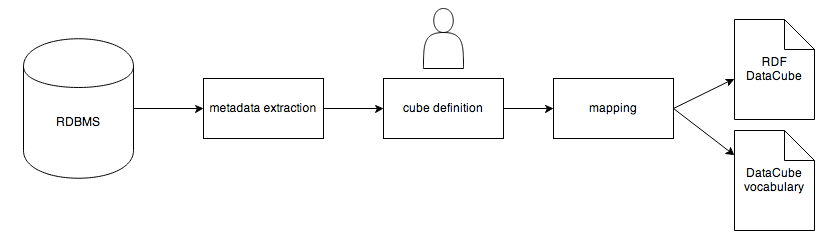
\includegraphics[width=140mm]{img/mapping-olap2dc.png}
	\caption{OLAP2DataCube mapping process}
	\label{fig:olap2dc-mapping}
\end{figure}


Let us take a brief excursion back to the OLAP2DataCube described in Section 
~\ref{rw:olap2dc}. The tool was not designed just to convert a non--RDF dataset 
into the RDF standard with respect to the DCV metaformat. Executing the tool on a 
dataset has one important side--effect: there is a new QB data structure definition
generated with bases on 
the structure of the input dataset. Therefore, the tool does not map the 
dataset to match an existing data structure definition, it creates a new one. That is definitely
needed when one transforms a non--RDF dataset into RDF. But once 
this is done, it is probable that a company or an organzation will produce the 
same kind of data periodically, therefore, they will reuse the same data structure definition.

This is the reason why we will propose a system which fill focus on the task of 
mapping the input dataset to match an existing data structure definition. 
The authors of the LDVM~\cite{ldvm} (see Section~\ref{sec:rw:ldvm}) propose to make standalone
visualizers. Each of them will 
be able to visualize a specific kind of datasets. Its visualization abilities will be described with
an \emph{input signature}. A Data Cube data structure definition could be easily transformed into
an example of such a signature. That is another reason why we want the tool to 
map the input dataset into an existing definition.

\begin{figure}
	\centering
	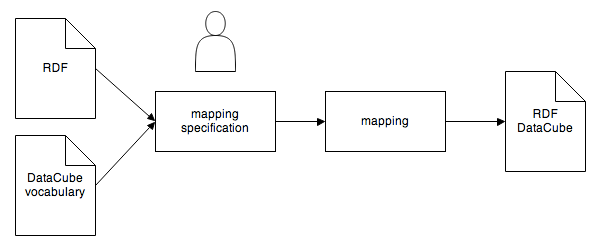
\includegraphics[width=140mm]{img/generic-mapping.png}
	\caption{RDF to DataCube mapping in a generic system}
	\label{fig:generic-mapping}
\end{figure}

That means we would like to enable the user to take an existing RDF
dataset and give it a statistical meaning. The initial thought was to
implement a set of specialized 
mapping modules. We would have to implement a standalone mapping module for
each existing Data Cube Vocabulary. Since this is rather impossible and 
surely inefficient, we made some experiments in order to ensure that we would be able to come 
up with a generic mapping component. That is why the process of the implemented
system will be similar to what is shown in Figure~\ref{fig:generic-mapping}. The 
process seen in the diagram represents a high--level view of the system. As we 
consider some additional criteria we will provide a more detailed schema of the 
proposed system. 

The biggest difference is that the original dataset can contain the statistical 
data in a not--so--obvious form, as in the case of the relational DB.
The user may need to apply an analytical 
extraction (a term introduced in~\cite{ldvm}) in order to select the transformed data.
We start with an arbitrary RDF document, 
specify the process of mapping and how the system transforms the data in order
to comply with the Data Cube Vocabulary standard. We also require the user to 
provide a Data Cube Vocabulary definition. The proposed system will map the data
to conform with such a definition.

We will now walk the reader through the decision process we have made in order to propose 
the system. As stated before, the input is an arbitrary RDF graph. To 
be able to map data from the graph to a form compliant with a Data 
Cube Vocabulary, the system also needs for a vocabulary to be a part of the input. 
As discovered in Section~\ref{datacube-vocabulary}, the vocabulary is another 
RDF graph.

Based on that fact, we concur that the system needs to contain a mechanism, which 
parses an arbitrary RDF graph and searches for DCV data structure definitions. 
We need to extract those definitions and have the user select one. The selected 
definition will be used in the upcoming steps to obtain mapping specification from 
the user. What we need to obtain is presented in 
Figure~\ref{fig:mapping-example}. On the right side the reader can see the 
generic visualization of a DCV data structure definition. A random graph is 
placed on the left side of the illustration. The dashed lines connect the resources 
from the original dataset with corresponding DCV components. Naturally, the 
figure represents an example of a mapping.

\begin{figure}
	\centering
	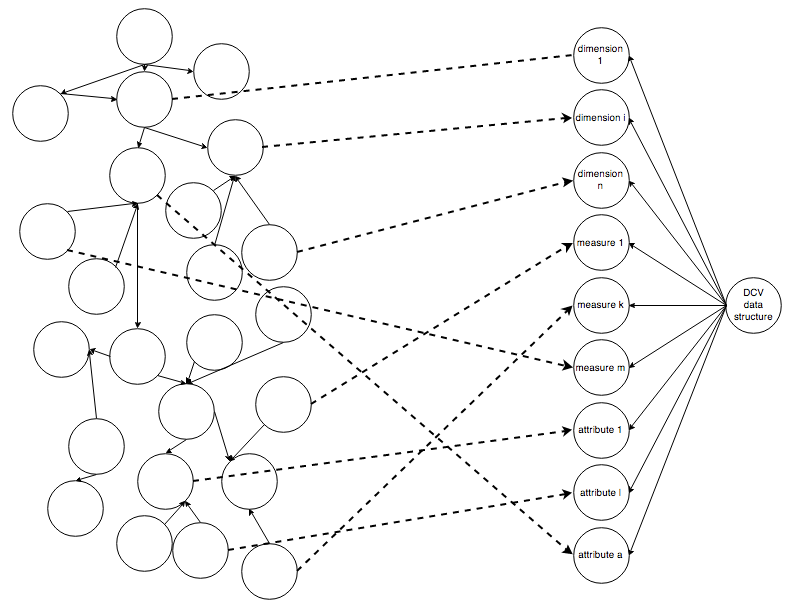
\includegraphics[width=140mm]{img/mapping-example.png}
	\caption{Mapping example. Original dataset on the left, DCV data structure definition on the right.}
	\label{fig:mapping-example}
\end{figure}

\section{Pattern selection}
We are lacking some rules telling the system how to do the mapping. 
Without such rules it is not possible to map the input graph properly. Let us 
imagine an input graph, for instance the whole DBPedia database. That represents a huge graph 
containing many facts and naturally, some of those are statistical data. But they 
are not referenced in such a context. For example the resource \emph{Prague}, which is the 
capital city of the Czech Republic has properties \texttt{populationTotal} and
\texttt{populationAsOf}. Together it creates a slice of a cube. This says that the 
city Prague (location dimension) had in a certain day (time dimension) 
a certain amount of citizens (measure).

Although this cube is originally based on a very simple pattern (a shape of a pair of cherries),
it is not possible to map such a slice into a form compliant with a 
data structure definition since the relation between the definition and the 
dataset is not defined in the original data. For a well--defined data structure 
definition and a well--defined dataset, it could be possible to propose another 
system, which would try to detect the relation and create them 
automatically. For instance, the location dimension, which is usually named
\emph{reference area} could be connected to a generic type -- a location.
Also the resource \emph{Prague} could be connected with the location type. But 
that would mean introducing a system, which would process a lot of data trying to 
match each supertype of the dimension with the properties of every resource in 
the graph. It would have to use advanced heuristics and it would probably have 
to adopt some techniques from the machine--learning field. A fully--automated 
system would also introduce a lot of mistakes into the results since it would 
be a highly experimental approach. Therefore, implementing such a system would 
not be the goal of this thesis. 

On the other hand, we would like to propose a system, which will be flexible 
enough to allow the user to take an arbitrary Data Cube Vocabulary data 
structure definition and map a reasonable part of this dataset into a compliant 
form.

Unfortunately, the phrase \emph{reasonable part} is not very scientific. 
It comes from the data semantics and it is quite difficult to formalize. What 
the user should map to a given data structure definition should have 
a corresponding semantics. For instance, if we use the population size example, the 
user should probably not map the statistics of government debts to that 
definition. Even though a country is a location, the amount of the debt represents a 
number and was certainly calculated on a specific day, therefore, the 
data match the ranges of the data structure definition components, but it does 
not match the semantics.

\begin{sloppypar}
On the other hand, we do not want to make the tool too restrictive in order to 
achieve better user experience. For instance, we have mentioned
(Figure~\ref{fig:example-dcv-dataset}) a data structure 
for the population example that declares a dimension \texttt{czso-ds-def:refArea}. 
The range of that dimension is specified as \texttt{czso-reg:Municipality}. 
With a restrictive approach, the tool would not enable the user to map the data from 
the DBPedia database to match the data structure definition, since the DBPedia 
dataset does not contain the \texttt{czso-reg} namespace. Nonetheless, Prague is 
certainly a Czech municipality. Therefore, the tool will not check the range 
while performing the mapping. If it had, the user would need to involve 
other datasets so as to provide the range--related information.
\end{sloppypar}

What is still missing is the way of informing the tool about how to map the data.
Obtaining such a specification can be implemented in many different ways. 
All of them are actually described in Chapter~\ref{chap:rw}. Some of the tools used 
their native language -- the SPARQL. That is beneficial for a developer due to 
its relatively easy implementation. But it is a bit cumbersome for a user 
who is required to know the SPARQL language. On the other hand, from all the approaches
it restricts the possibilities of the system the least. It enables the user 
to specify a wide range of mappings.

OLAP2DataCube took an advantage of the database structure (Section ~\ref{olap2dc}) --- 
especially of relational feature --- foreign keys. Since the RDF format 
is based on expressing relations it would not present an issue. But what the 
OLAP2DataCube tool did, was that it transformed already existing statistical data from
the star--shaped database structure into another format. But in the world of RDF 
data we would restrict the tool a lot if we relied only on star--shaped 
schemas, hence, we need to work with a generic graph.

Tabels introduced a custom DSL that should have made the situation easier for 
a user (Section~\ref{rw:tabels}). But as experienced while doing research for Chapter~\ref{chap:rw}, 
we did not find it very user--friendly. There certainly was a pre--generated script based
on the uploaded file but in most cases the user had to modify the script in order to
achieve desired results. The user is required to learn a 
completely new language, but will probably not find any other use of such a skill
elsewhere. Moreover, it is not an easy task to implement the 
custom DSL itself. Therefore, we consider this approach to be the worst.

The last approach we have noted is the \emph{query--by--example} introduced in 
Tabulator (Section~\ref{sec:rw:tabulator}). It was used to let the user specify what type of data patterns they are 
interested in. In the exploration mode the user was able to \emph{visually} 
specify the pattern and switch to the analytical mode. Such an approach enables 
us to construct a SPARQL query and come closer to the very first (and the least restrictive) 
approach. Nonetheless, it brings some new implementation issues.

The most obvious one is the transformation of the user's selection into a SPARQL query. 
We will also require the system to be capable of making a preview of the 
original dataset in order to offer the user a visualization. The visualization 
itself will interact with the user and provide them a way to specify the pattern.

Of course, the query--by--example does not need to be necessarily done visually. But 
obtaining an example with a non--visual approach leads to the involvement of a DSL. Even 
a simple DSL, for instance a variation of CSV format, is not as user--friendly as 
the visual approach. The visual approach also enables us to force some 
restrictions to avoid dealing with an arbitrary user input. We will 
obtain an input that is already valid.

After obtaining the pattern all the necessary information are gathered. We 
may proceed to the mapping process itself. The mapping module will query the 
data source for the data. It will use the pattern specified by the user. After 
fetching the data, it will construct a new graph containing a set of DCV 
observations. Based on what we have learnt so far, the system will appear in detail 
as shown in Figure~\ref{fig:generic-mapping-detail}.

\begin{figure}
	\centering
	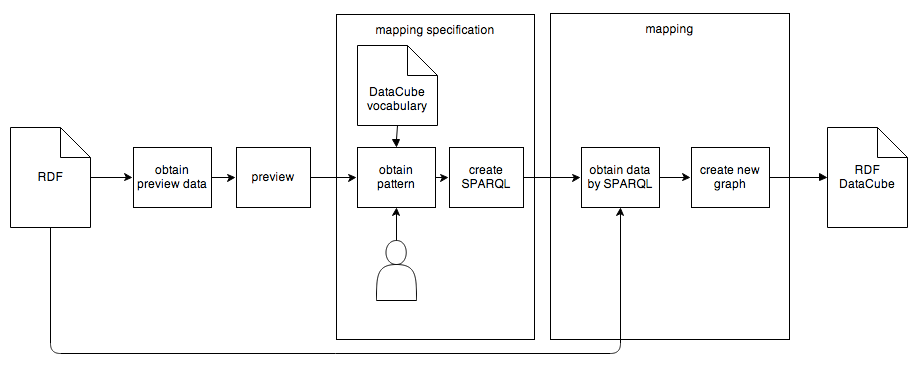
\includegraphics[width=140mm]{img/generic-mapping-detail.png}
	\caption{Detail of the proposed system.}
	\label{fig:generic-mapping-detail}
\end{figure}


\section{Mockups}
\FloatBarrier
We will show the reader our idea of a user interface of the proposed system. We 
will refine some previously outlined features, especially the pattern selection.

In the first step (Figure~\ref{fig:mockup-01}), the user is required to specify the source of the data that 
will be transformed. They will probably supply a reference to a SPARQL Endpoint,
e.g. \url{http://dbpedia.org/sparql}. The user also has to reference a graph, which contains the 
desired Data Cube Vocabulary data structure definition.
That is a URL as well, e.g. \url{http://datacube.payola.cz/dsd/population.ttl}.
The type of data source 
is needed in order to determine how to fetch the data.
\begin{figure}
	\centering
	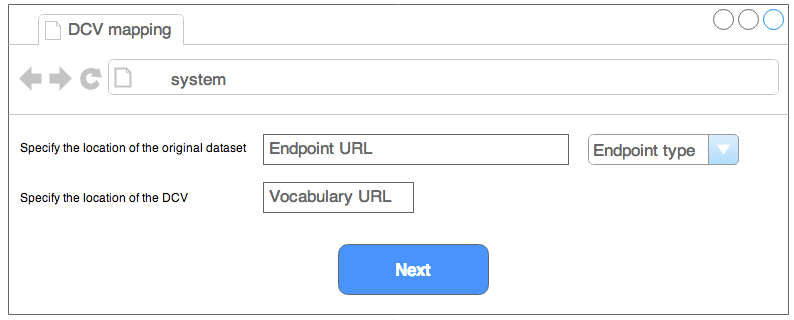
\includegraphics[width=120mm]{img/mockup-01.png}
	\caption{Step 1: data source and vocabulary specification}
	\label{fig:mockup-01}
\end{figure}

After proceeding to the next step (Figure~\ref{fig:mockup-02}),
the user will be asked to choose a DCV data 
structure definition. The definition list is prepared based on the vocabulary provided 
in the previous step. The system has already parsed the supplied graph and filtered all
DCV data structure definitions. As an example, the user will select the
\url{http://datacube.payola.cz/dsd#PopulationSizeDefinition} data structure definition.

\begin{figure}
	\centering
	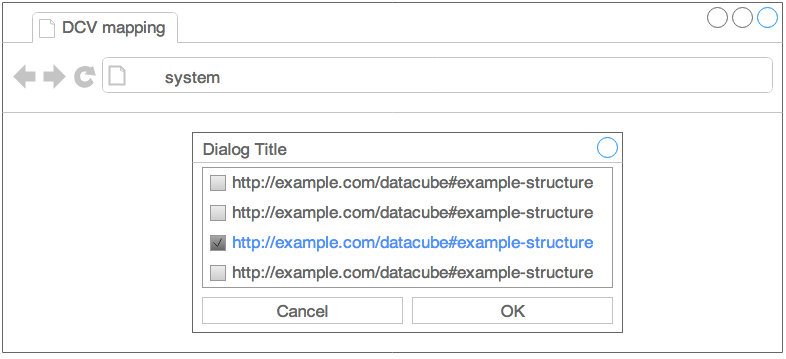
\includegraphics[width=120mm]{img/mockup-02.png}
	\caption{Step 2: DCV data structure selection}
	\label{fig:mockup-02}
\end{figure}

The system now selects data for a preview. The retrieved dataset is 
visualized and shown in a dialog (Figure~\ref{fig:mockup-03}). The user is 
required to specify a pattern. The specification is done by clicking the vertices in 
the visualized graph (some progress is shown in Figure~\ref{fig:mockup-05}).

\begin{figure}
	\centering
	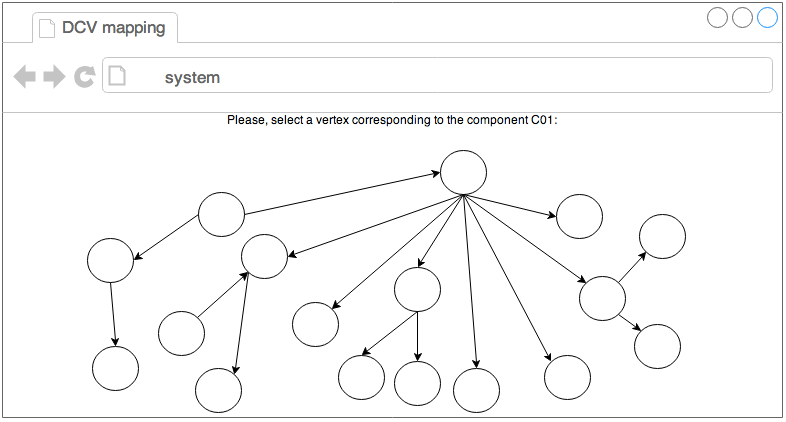
\includegraphics[width=120mm]{img/mockup-03.png}
	\caption{Step 3: Pattern selection}
	\label{fig:mockup-03}
\end{figure}
\begin{figure}
	\centering
	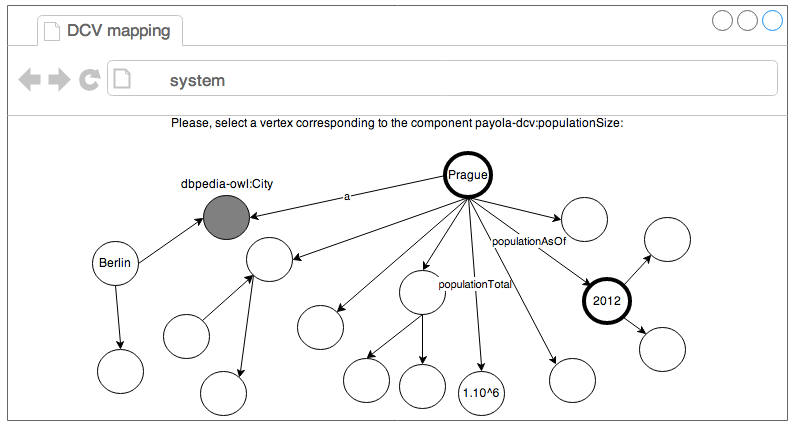
\includegraphics[width=120mm]{img/mockup-05.png}
	\caption{Step 3 (example): Pattern selection. The user has to provide an example
	for mapping the dataset to a population vocabulary. In the last step, the user is asked
	to select a vertex corresponding to the \texttt{payola-dcv:populationSize} property.
	They have already selected the vertices representing Prague and observation date
	in order to satisfy the other components. The \texttt{dbpedia-owl:City} vertex can
	be selected to refine the example, but it does not correspond with any component.
	The user is about to select the vertex connected via the \texttt{populationAsOf} 
	relation. This represents an example of selecting a meaningful pattern, which 
	is a connected graph.}
	\label{fig:mockup-05}
\end{figure}

After the pattern is specified the system has all the information it needs. The 
user is able to start the mapping process. When done, the system offers
the results (RDF graph).
\FloatBarrier

\section{Benefits of integration into Payola}
\label{why-payola}
Since we have participated on the implementation of the Payola RDF tool, we will 
now go through the pros and cons of integrating the proposed system into Payola.
We will also decide if we proceed with the integration.

In Chapter~\ref{ch:payola} we familiarized the~reader briefly with the~main
concepts of the~Payola framework. The reader also knows how the~analyses
evaluation is done. Therefore we may demonstrate the benefits arising from
the integration of the proposed system with the Payola framework.

The crucial feature of the Payola framework is the analysis subsystem. It enables a user
to combine multiple data sources and benefit from their 
combination. Based on that, a completely new set of facts can be computed.
(This could be optimized with SPARQL 1.1 and Federated queries~\cite{federated-queries}.) 
Therefore, it could be handy to introduce a Data Cube Vocabulary analytical 
plugin, which would be able to convert the results of an analysis into the Data 
Cube Vocabulary format. Such a plugin could be connected directly to an output
of a data fetcher plugin --- this will cover the basic implementation shown in 
Figure~\ref{fig:generic-mapping-detail}.

But we can go a bit further. Since it would be an analytical plugin, the user 
would be able to use such a plugin in an arbitrary step of the analysis. Let us look back again
at the DBPedia and the population statistics example. A plugin representing the proposed
system would substitute multiple different plugins 
in order to obtain the same data. In this case it is the \texttt{Typed}
plugin and the \texttt{Property selection} plugin. Those are covered based on the selected pattern.
In addition, the result would be 
compliant with the Data Cube Vocabulary standard.

Another asset is considered to be the ability to transform multiple data 
sources in one step. The users might also further use the converted datasets --- combine them
(join, union) and analyze those datasets in a unified format (specified by the DCV).

The next benefit of the integration with the Payola analyzer is that the user 
can assemble an algorithm, which is applicable multiple times. The main 
advantage is that it reflects the current state of the data sources at
the time of the execution. That means that if the data source contents get 
updated, the user just executes the analysis again and the mapping is instantly 
performed. There is no need to specify anything for the second time.
This is useful especially in a case where the analysis is more complicated than the 
mapping process itself.

As stated before, the Payola application also offers the functionality of 
sharing. This feature is usable at least in a case of sharing the results 
of an analysis. The introduction of a Data Cube Vocabulary plugin does not change anything.
The user will still be able to share the analysis. If the analysis contains just the data fetcher 
and the DCV plugins, the user shares only the mapping process.

Another aspect could be an effort needed to implement such a system. Since the 
goal of software engineering is not to implement the same systems over and over 
but to bring new systems, new features, speed up the computation process and 
bring better user experience, it makes no sense not to take advantage of 
an already existing platform. The same approach could be seen in the case of reviewed 
tools like Olap2DataCube (section~\ref{olap2dc}) or CubeViz 
(section~\ref{cubeviz}).

The Payola framework contains a variety of useful components. As an example of 
such components we might name data fetchers, RDF processing modules or 
visualization API.

Since a part of the goal of this thesis is to implement an exemplary 
visualization that takes advantage of the Data Cube Vocabulary format, it will 
be very useful to stay focused on the task and implement just the visualizer, 
instead of a lot of supporting subsystems that are already 
implemented elsewhere.

Moreover, we can take advantage of the existing visualization plugins. The basic 
one, triple table plugin, offers a quick overview of the data. The user 
will also be able to download the results of the transformation into a static 
RDF file for further use or just for simple backup purposes.

\begin{figure}
	\centering
	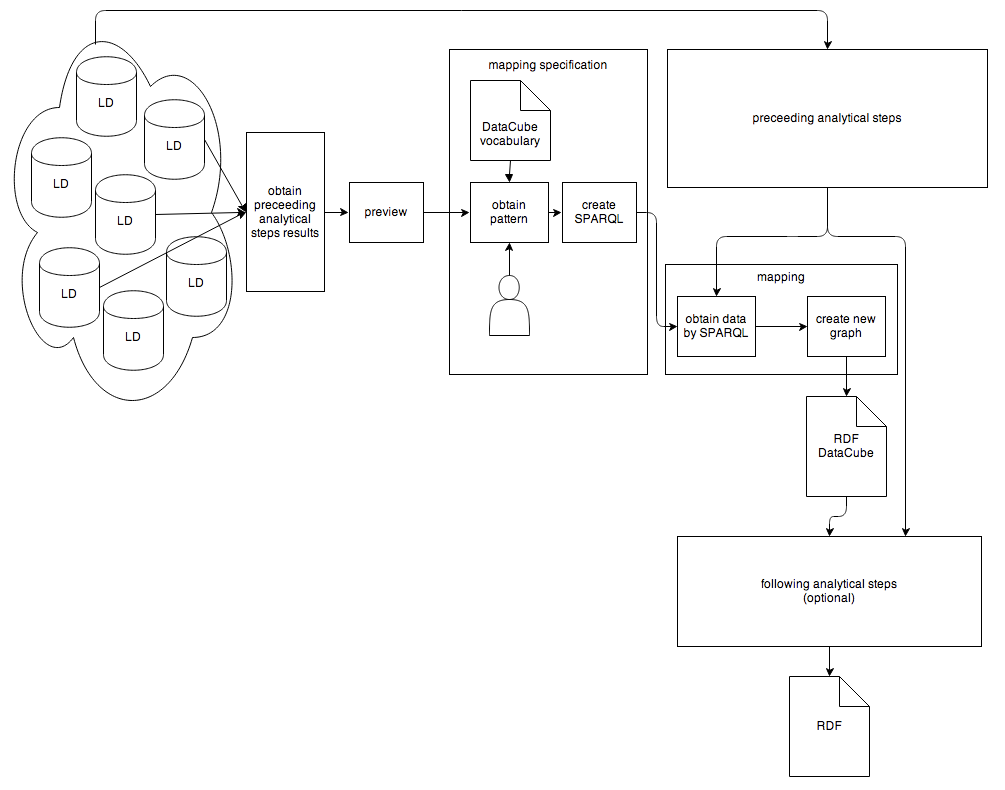
\includegraphics[width=140mm]{img/payola-mapping.png}
	\caption{Mapping process integrated into the Payola analyzer.}
	\label{fig:payola-mapping}
\end{figure}

We show a possible way of the integration of the mapping process into the Payola analytical extraction
in Figure~\ref{fig:payola-mapping}. It shows the proposed system in a context of an
analytical pipeline. Such a pipeline is constructed by the user. The process starts with querying data 
sources in order to offer the user an overview. The amount of the sources depends 
on which sources are involved in the analytical pipeline. They are fully independent 
and spread throughout the whole Internet. The obtained data are visualized to 
the user who is required to select a pattern. Since we need to guide the user 
to select a proper one, we also need them to specify a Data Cube Vocabulary. 
We will need to parse the Vocabulary, extract the DCV datastructure definitions 
and offer the user a list of the available definitions. After they choose one, we will be able to determine how many mapping references we need the 
pattern to contain. The number is, of course, based on the amount of components 
within the datastructure definition. We will construct a SPARQL query based on the selected pattern.

The rest of the process is a common analytical pipeline execution. The Data Cube 
Vocabulary plugin can be interpreted as a standard plugin. Since the 
transformation is done by executing a SPARQL query, it corresponds with an 
execution of a SPARQL query plugin. During the evaluation of the analytical pipeline we reach a certain point of an undergoing mapping (thanks to a DCV plugin). On the output of this plugin, we will for certain find a dataset compliant with the DCV standard. But the dataset need not 
be the result of the analytical pipeline execution. It may be used as an input 
for the upcoming analytical steps.

Based on facts presented in the text above we find it reasonable to integrate 
the proposed system into Payola.

\section{Formalization}

In this section, we are going to formalize the aforementioned process a bit 
more. We need to specify the input of the system. We will also 
provide a definition of the mapping process. A description of the output will be 
also presented.

\subsection{Input and output}

The input of the system will be an arbitrary RDF graph $G_{input}$ as shown
in Figure~\ref{fig:mapping-example}. It will be mapped into a form compliant
with the DCV standard. Since the DCV also takes advantage of the RDF standard,
the result will likewise be a graph, let us say $G_{output}$.

\begin{figure}
	\centering
	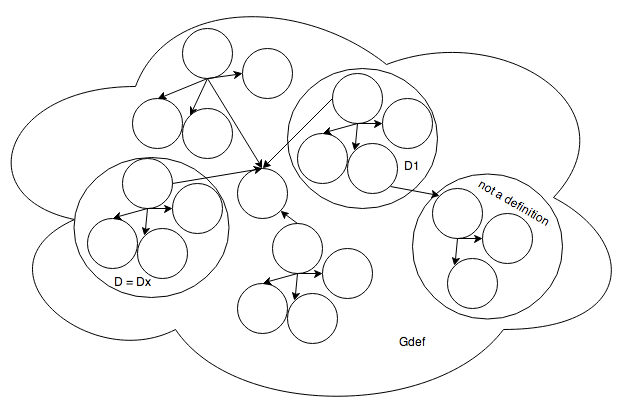
\includegraphics[width=120mm]{img/definition-in-graph.png}
	\caption{A user will provide an arbitrary RDF graph $G_{def}$, which may contain more than one definition. The user will select only one to work with, $D$.}
	\label{fig:definition-in-graph}
\end{figure}

As stated before, the system will have another input --- a data structure 
definition. The Data Cube Vocabulary standards are built on top of the RDF as described in the 
section~\ref{datacube-vocabulary}. That means, that a data structure is also a 
graph. We will denote the user--provided definition as $D$. But the user will probably not 
supply just a definition. They will provide an arbitrary graph, which contains the definition $D$ 
(or even more definitions) as a subgraph (see Figure~\ref{fig:definition-in-graph}).
We will denote a graph
supplied by the user as $G_{def}$. The system has to extract a list of all the definitions
(let us say $D_1, ..., D_d$) from the graph $G_{def}$. As shown in Figure~\ref{fig:mockup-02},
the user will select one of the offered definitions, for instance $D = D_x (1 \leq x \leq d)$.
The graph may contain also other data, not only DCV definitions. It is true 
that:\\

{\centering $D \subseteq G_{def}$ \\[0.5cm]}

But having the graphs $G_{input}$ and $D$ 
is not enough. We require the user to specify also an example pattern (based on the
query--by--example principle). Since all the inputs and outputs are RDF
graphs ($G_{input}$, $G_{def}$, $D$, $G_{output}$), we can take 
advantage of some existing approaches specialized on RDF transformation. 
A technically simple but powerful way, is to utilize the SPARQL language. Based on what we have introduced before, we are able to transform a user--selected pattern into a form of a SPARQL
query. We will talk about such a query as of a \emph{transformation query} and denote it $Q_t$.

What we have now is an information about what is needed on the input and 
what the result would be:

{\centering $(G_{input}, G_{def}, Q_t) \rightarrow G_{output}$ \\[0.5cm]}

In fact, the user will make the selection of the definition $D$ before the 
mapping starts. Therefore, we can extract the definition $D$ from the 
generic graph $G_{def}$ and use it as a part of the input. That is possible because 
the system does not require an arbitrary RDF graph $G_{def}$. It requires the DCV 
data structure definition $D$. The rest is done in order to improve the user 
experience. Therefore:\\

{\centering $(G_{input}, G_{def}, Q_t) \rightarrow (G_{input}, D, Q_t) \rightarrow G_{output}$  \\[0.5cm]}

What we still do not have is a description of the SPARQL query used to transform the 
data in order to obtain the output graph $G_{output}$. The form of the query is dependent on the 
definition $D$. To be more accurate, the definition $D$ contains
a set of components ($C_1, ... , C_n$), which represents dimensions, measures and attributes. Let us say, that the 
structure has defined $n$ components, $m$ measures, $d$ dimensions and $a$ 
attributes. It is true that\\

{\centering $n = m+d+a$ \\[0.5cm]}

For each n--tuple matched in $G_{input}$, the output graph $G_{output}$ will contain a node with $n+2$ 
neighbours (+1 for \verb|qb:Observation| and +1 for \verb|qb:dataSet| --- first two statements
in Figure~\ref{fig:output-graph}). A concrete example of an observation is shown 
in Figure~\ref{fig:output-graph-instance}.

The result will comply with the template shown
in Figure~\ref{fig:output-graph}. $O_i$ denotes an identifier (URI) of the generated 
observation, $S$ stands for an identifier of the input dataset,
$T_{Dim_1}$~...~$T_{Dim_d}$ stands for the type of a corresponding dimensions 
from the given data structure definition, similarly for
$T_{Msr_1}$~...~$T_{Msr_m}$ -- measures and
$T_{Attr_1}$~...~$T_{Attr_a}$ -- attributes. $R_{i,1}$~...~$R_{i,n}$ stands for
resources matched in the input graph $G_{input}$, moreover, it means that the value 
of the dimension $T_{Dim_1}$ is $R_{i,1}$, etc.

\begin{figure}
  \centering
  \begin{tabular}{lll}
$O_i$~~~~~~~~~~~~& a~~~~~~~~~~~~~~~~~~~~~~~~~& qb:Observation ;\\
          & qb:dataSet    & $S$ ;\\
          & $T_{Dim_1}$ & $R_{i,1}$ ; \\
          & $...$              & $...$ \\
          & $T_{Dim_d}$  & $R_{i,k}$ ; \\
          & $T_{Msr_1}$  & $R_{i,l}$ ; \\
          & $...$              & $...$ \\
          & $T_{Msr_m}$ & $R_{i,m}$ ; \\
          & $T_{Attr_1}$  & $R_{i,o}$ ; \\
          & $...$              & $...$ \\
          & $T_{Attr_a}$  & $R_{i,n}$ . \\
\end{tabular}
\caption{Description of an output graph node (turtle notation)}
\label{fig:output-graph}
\end{figure}

\begin{figure}
  \centering
  \scriptsize
  \begin{tabular}{lll}
\textless http://ex.com/observed\#1234\textgreater & a& qb:Observation~;\\
          & qb:dataSet    &  \textless http://dbpedia.org/sparql\textgreater ~;\\
          & my-population:count & '10233222' ; \\
          & my-population:location & \textless http://dbpedia.org/page/Prague\textgreater ~;\\
          & my-population:time  & '2012-02-23' . \\
  \end{tabular}
\caption{A concrete instance of the pattern shown in Figure~\ref{fig:output-graph}}
\label{fig:output-graph-instance}
\end{figure}

\subsection{Transformation query}

The last unanswered question is how the query $Q_t$ should look like. 
It would certainly not be an arbitrary query. Let us analyze the situation and 
walk the reader through the process of coming up with a set of constraints for the 
query.

It should be obvious that the query $Q_t$ will generate a new graph
(in fact, it will generate the graph $G_{output}$) based on some specific rules
(see Figure~\ref{fig:mapping-example}). 
Therefore, it would be a CONSTRUCT query. It is also very clear what kind of 
triples it will generate; the pattern is shown in Figure~\ref{fig:output-graph}.
The only thing we need to sort out is retrieving the resources $R_{i,1}, ... R_{i,n}$.

\subsubsection{Pattern}
\label{sec:pattern-definition}
The process of resolving those resources depends on the input graph $G_{input}$.
We will demonstrate it on the most simple case --- a 2--dimensional data structure 
definition. Such a definition requires us to specify how to select a 3--tuple of resources from 
the graph (2 dimensions, 1 measure).
We will present some ideas while using the example of the population size.

The initial idea could be that we need a country, therefore, we map all the 
countries to the \texttt{refArea} dimension, all instances of time to the \texttt{refPeriod} 
dimension and all instances of \emph{numbers} to the measure. But that is not sufficient. At first,
we need to make sure that all instances of numbers 
really express an amount of citizens in a country. Moreover, we need to map the
matching amount of citizen to a corresponding country. Therefore, all the 
selected resources need to be connected with the rest. We need to select a 
specific pattern, which will contain the relation between the resources.

\begin{figure}
	\centering
	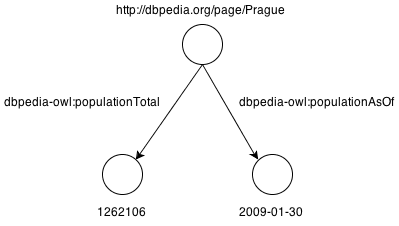
\includegraphics[width=80mm]{images/cherry.png}
	\caption{Cherry--shaped pattern example.}
	\label{fig:cherry}
\end{figure}

\begin{figure}
	\centering
	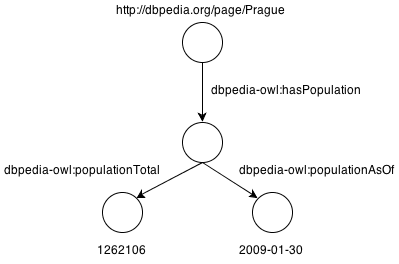
\includegraphics[width=80mm]{images/cherry_blank.png}
	\caption{The example from Figure~\ref{fig:cherry} extended with a blank node.}
	\label{fig:cherry-blank}
\end{figure}

We will use an example from DBPedia, 
the Czech Republic resource. The resource itself reference to a location, 
therefore, it should be mapped to the \verb|refArea| dimension. It has got a 
\verb|populationTotal| property, which should be mapped to the measure. Last, but not 
least, it has the \verb|populationAsOf| property, which should be mapped to the 
\verb|refPeriod| dimension.

That gives us a simple shape of a cherry--pair as shown in
Figure~\ref{fig:cherry}. But what 
if the resource us connected to a blank node with an edge of type 
population and the blank node has two properties --- size and time
(see Figure~\ref{fig:cherry-blank})?
It is clear now that there could be in the least a long oriented path between the participating 
vertices.

While keeping this fact in mind, we can accede to assembling a formula of a generic pattern used for an extraction of the resources from the original graph $G_{input}$. But 
there is one piece of a puzzle still missing. While analyzing all the
possibilities, until now we assumed that the pattern \emph{starts} (in the topological order)
with a resource, which represents one of the data structure components. But that is not  
the case.

The most simple example is the observation pattern itself. The 
entities come together but their connection is dependent on a completely 
different resource. We reference such an entity
as a \emph{reference vertex}. Any pattern vertices corresponding to a component from the 
data structure definition could also match the \emph{reference vertex}.

Later on, we have discovered that such a kind of patterns is not what the user 
wants to select. We have applied too much restrictions. Such a pattern
represents only a subset of patterns the user may want to select. We have learnt
that the most concrete designation of such a pattern is the well--known term:
\emph{connected graph}.

We left out the term \emph{oriented} on purpose. While experimenting with the 
system, we had discovered that for purposes of the pattern specification the 
orientation is not necessary. We need all the referenced vertices to have a 
relation between each other, but the orientation does not matter.

In order to get the reader familiar with some 
approaches we will utilize while implementing the system, we are about to point 
out some facts.

We are about to build a pattern $P$. The pattern reflects an example set by the user,
an example that represents the user’s proceedings of the data mapping to the components from a data structure definition. The pattern will
be used later to construct the desired
transformation query $Q_t$. As shown in Figure~\ref{fig:mapping-example}, we 
require the user to find an equivalent for each component ($\{C_1, ... C_n\}$) of the data
structure definition $D$ in the input graph $G_{input}$. The equivalent for $C_1$ is in 
Figure~\ref{fig:output-graph} denoted as $R_{i,1}$. But there are many other 
equivalents for the component in the input graph ($R_{i,1}$ is one of many instances). 
That is why we need to generalize the symbols used for matching 
resources. Therefore, we introduce a new set of symbols, $M_1, ..., M_n$ to 
express that such a resource is a vertex matched in the mapping process, $M_1$ 
for component $C_1$, etc. To understand this better, see Figure~\ref{fig:mapping-pattern}}.

\begin{figure}
	\centering
	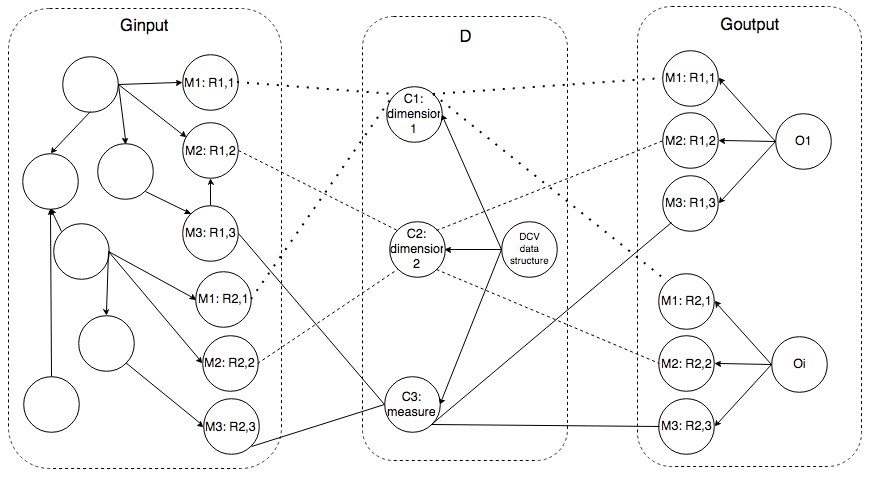
\includegraphics[width=140mm]{img/mapping-pattern.png}
	\caption{An example of mapping. $G_{input}$ is an input graph, $D$ a data 
	structure definition, $G_{output}$ an output graph. Lines between those graphs represent mapping.
	For each component $C_1, ..., C_n$ we need the user to give an example of a matching entity.
	That means one concrete instance $R_{i,1}$ for component $C_1$. Such match is generally denoted
	as $M_1$.}
	\label{fig:mapping-pattern}
\end{figure}

Please, keep in mind that we are about to construct a 
connected graph. Therefore, we define an invariant, which says that in every 
step of the pattern construction the pattern $P$ needs to be a connected graph.

As shown in Figure~\ref{fig:mockup-03} and Figure~\ref{fig:mockup-05},
the system iterates over data 
structure definition components and lets the user select an example of a 
vertex corresponding to the current component.

For each component we are about 
to extend the constructed pattern. We will take advantage of the notation from the
graph theory, because the pattern is also a graph (let us remember the connected graph invariant).
Therefore, in the beginning:\\

{\centering $P = (V = \emptyset, E = \emptyset)$ \\[0.5cm]}

We will extend the pattern $P$ for each component $C_1, ..., C_n$ of the 
definition $D$. We need the pattern to contain all the vertices from $\{M_1 ,..., 
M_n\}$, because they represent examples of each component. An example of
a pattern extension for a component is shown in 
Figure~\ref{fig:pattern-enhancement}.

In order to maintain the invariant, we will enable the user to add only such 
vertices that are somehow related with an arbitrary vertex already contained in 
the pattern $P$ (an element of set of vertices $V$ --- vertices $a,b,c,d$
in Figure~\ref{fig:pattern-enhancement}, step 1).
To make it more formal, let us remind the reader that an edge is a tuple 
of vertices (e.g. $(v_1,v_2)$). In case of an oriented graph, it depends on the order within 
the tuple.

Therefore when adding an arbitrary vertex $v_i$, we demand that there exists an 
edge $e$ for which it is true that:

\begin{center}
{$e = (v_i,v_x)$ or $e = (v_x, v_i)$ \land $v_x \in V$ \\[0.5cm]}
\end{center}

\begin{figure}
	\centering
	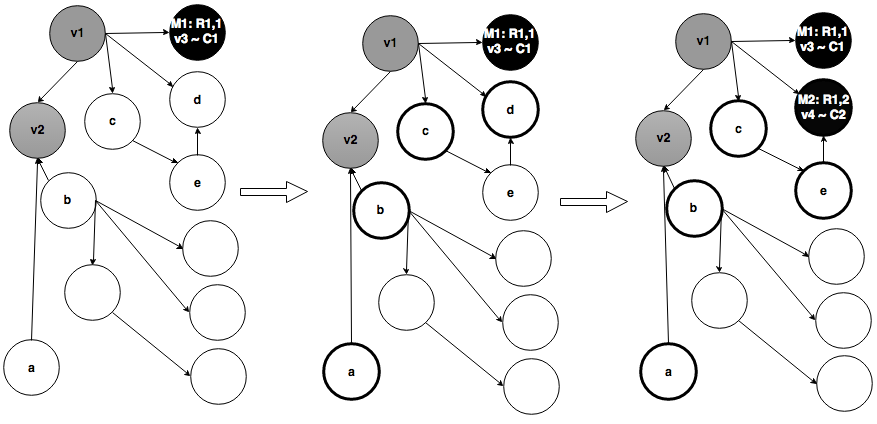
\includegraphics[width=140mm]{img/pattern-enhancement.png}
	\caption{An example of pattern extension. We start with three selected vertices
	-- $v_1, v_2, v_3$. Due to the invariant, we are able to extend the pattern only with
	the vertices $a,b,c,d$. We choose the vertex $d$.}
	\label{fig:pattern-enhancement}
\end{figure}

Of course, this is not possible to apply in the first step since the graph $P$ is empty. 
In order to make the pattern more accurate or more restrictive to obtain a more 
efficient transformation query, the user may want to reference some other 
vertices and not only the component equivalents.
Because of that observation, for each component from $C_i \in \{C_1 ,..., C_n\}$ the pattern is 
extended by adding a set of vertices $V_i = \{v_{i_1}, ..., v_{i_u}\}$ and set of corresponding edges 
$E_i$:\\

{\centering \forall $C_i \in \{C_1 ,..., C_n\}$: $P = (V = V \cup V_i, E = E \cup E_i)$ \\[0.5cm]}

In Figure~\ref{fig:pattern-enhancement} we make two steps. In the first one, we 
can add vertices $a,b,c,d$ and we choose to add $d$. That means that we extend 
the set of vertices $V$ with the set $V_i = \{v_4 = d\}$ and the set of edges $E$ with 
the set $E_i = \{(v_1,v_4 = d)\}$.

Because of the invariant:\\

{\centering $\exists e \in E_i: e = (v_{in}, v_{out}) \land (v_{in} \in V \lor v_{out} \in V)$\\[0.5cm]}

and of course:\\

{\centering $M_i \in V_i \subseteq V$ \\[0.5cm]}

--- the example equivalent $M_i$ for component $C_i$ was also selected. One of the 
added vertices from $V_i = \{v_{i_1}, ..., v_{i_u}\}$ is equal to $M_i$ ($v_3$ is equal to $M_1$
in Figure~\ref{fig:pattern-enhancement}).
   
By applying the described approach, we get a connected graph, where:\\

{\centering $\{M_1, ..., M_n\} \subset V$ .\\[0.5cm]}

That means, that the pattern covers our needs. Now, we are about to present
a generic form of the pattern, which will come out from 
such an approach. The pattern is shown in Figure~\ref{fig:sparql-pattern}. 
$n$ of the vertices from the $\{v_1, ..., v_v\}$ matches vertices $M_1, ..., M_n$.

\begin{figure}
\begin{Verbatim}[commandchars=\\\{\},codes={\catcode`$=3\catcode`_=8}]
  CONSTRUCT \{
    []   a   <http://purl.org/linked-data/cube#Observation> ;
         <http://purl.org/linked-data/cube#dataSet>   $S$ ;
         $C_1$      $M_1$ ;
         ...   
         $C_i$      $M_i$ ;
         ...   
         $C_n$      $M_n$ .
  \} WHERE \{
    \{
      SELECT DISTINCT ?$M_1$ ... ?$M_n$
      \{
         $v_1$     $E_1$     $v_2$
         $v_2$     $E_2$     $v_3$
         ...
         $v_{i-1}$   $E_{i-1}$    $v_i$
         $v_i$     $E_i$      $v_{i+1}$
         ...
         $v_{v-1}$   $E_{v-1}$    $v_v$
      \}
    \}
  \}
\end{Verbatim}
\caption{Pattern of the transformation SPARQL query}
\label{fig:sparql-pattern}
\end{figure}

\section{Visualizers}
In the beginning, we promised to implement an exemplary visualization.
Unfortunately, the Data Cube Vocabulary standard covers a wide variety of data domains, 
therefore it is hard to make a decision and choose, which visualization should be offered.

Based on what we have seen while exploring tools described in 
Chapter~\ref{chap:rw} and keeping in mind the rules of a so--called 
\emph{visualisation mantra} (Section~\ref{sec:rw:mantra}}), we decided to implement two visualizers, 
TimeHeatmap and Universal DCV. 

\subsection{TimeHeatmap}
The decision to implement this visualizer was based on the example of the population size data
presented in Chapter~\ref{ch:statistical-data}. A table or a bar chart is 
definitely a reliable way of presenting this kind of data. But while getting 
familiar with Data Cube Vocabulary, we found out that it is very popular to 
visualize geospatial data. A visualization on a map is easy to understand and is
very popular among the non--technical people. It helps to popularize Data Cube 
Vocabulary. This is also the correct type of visualization for data journalists we 
have mentioned before.

As the name suggests, this visualizer is able to handle datasets with two 
kinds of dimensions. The first one will express the time of the measurement, the 
second one will cover its location. It will support one measure that has to be 
a number.

We will place a heatmap layer over a standard map layer. The layer will express 
the intensity of the measured value in respect to the others. The scale will go from 
green to red where the latter represents the largest value measured.

\subsection{Universal DCV}
Implementing a domain--complete library of visualizers is a long--term project. 
Despite the fact, we would like to offer a visualizer, which would enable the 
user to visualize a large amount of datasets in a comfortable way. While
experimenting we have experienced on our own some discomfort in reading triple tables.

That is why we have decided to implement a visualizer, which takes advantage of 
the idea behind faceted browsers. We presented some of those in 
Chapter~\ref{chap:rw}. Therefore we would like to implement a visualizer that will 
enable the user to slice visualized datasets and prepare usual visualizations of 
the slices. A mockup of such a visualizer is shown in 
Figure~\ref{fig:dcv-universal}. It should contain a pie chart and a bar chart 
visualization.

\begin{figure}
	\centering
	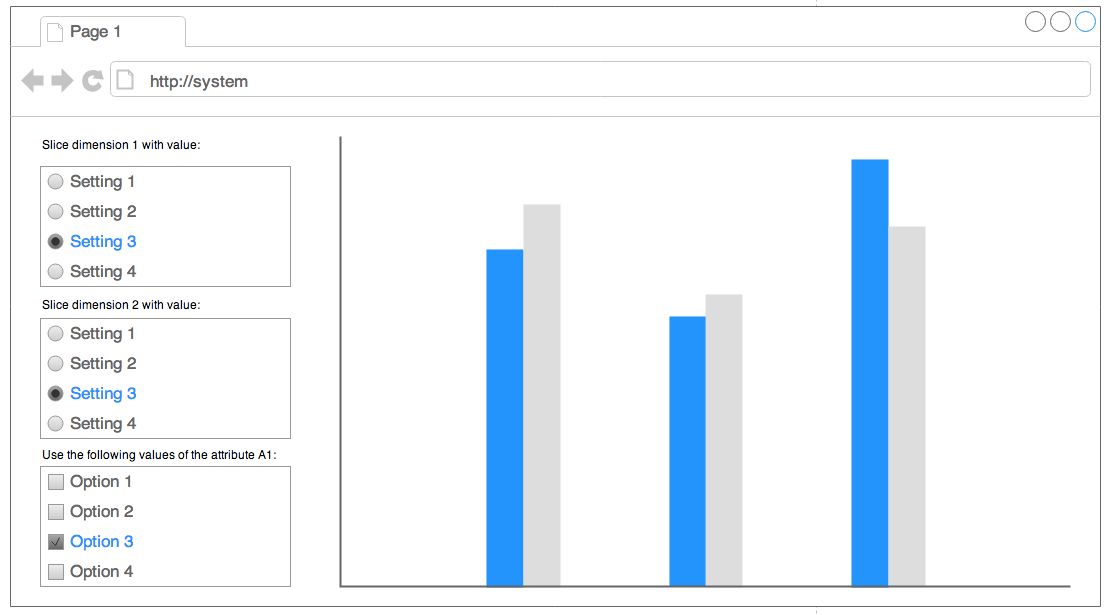
\includegraphics[width=140mm]{img/dcv-universal.png}
	\caption{Data Cube Vocabulary universal visualizer.}
	\label{fig:dcv-universal}
\end{figure}



